
\documentclass[xcolor=table, xllnames]{beamer}

\mode<presentation> 

\usetheme{Madrid} 

\usepackage{graphicx} 
\usepackage[labelformat=empty]{caption}
\usepackage[spanish, USenglish]{babel} 
\usepackage[utf8]{inputenc}
%\usepackage{movie15}
\usepackage{multimedia}
\usepackage{media9}
\usepackage{hyperref}
\usepackage{tikz}
\usepackage{verbatim}
\usepackage{color}
%\usepackage[x11names,table]{xcolor}

\selectlanguage{spanish}

\title[]{Estudio in silico de la din\'amica espacio-temporal de la somitog\'enesis} 

\institute[] {
{\large Examen de Doctorado} \\[.2cm] 
%Protocolo Doctorado \\[.1cm] 
Presenta: Jes\'us Pantoja Hern\'andez \\[.2cm]

\begin{tabular}{rl}
	Tutor:   & Dr. Mois\'es Santill\'an Zer\'on \\ 
	Sinodales:& Dr. Jes\'us G. Rodr\'iguez Gonz\'alez\\
			  & Dr. Daniel P. S\'anchez  Herrera\\
			  & Dr. Bruno A. Escalante Acosta\\
			  & Dr. V\'ictor F. Breña Medina \\
			  
\end{tabular}

}

 \date{13 de julio 2021}

\begin{document}
%--------------- Portada
\begin{frame}
\titlepage % Print the title page as the first slide
\end{frame}


%------------Diapositiva 2
\begin{frame}
	\frametitle{Introducci\'on} 
	\begin{tabular}{ccc}
		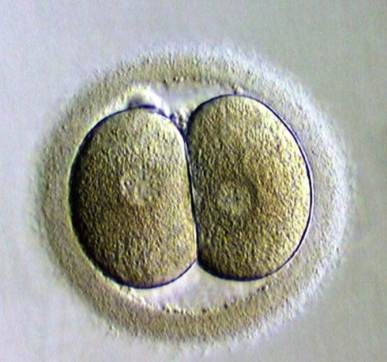
\includegraphics[width=3.6cm]{Figuras/seg1.jpg} & %\pause
		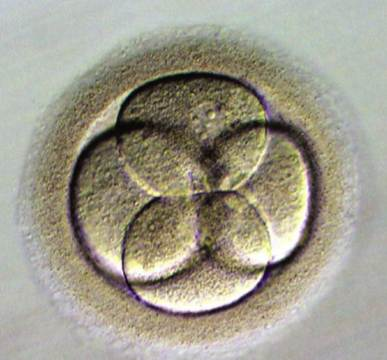
\includegraphics[width=3.6cm]{Figuras/seg2.jpg} & %\pause
		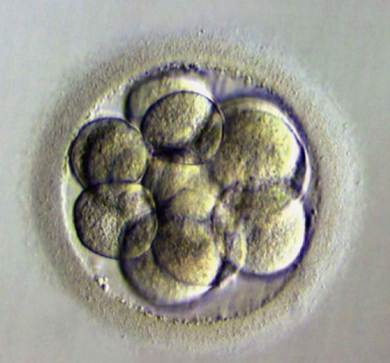
\includegraphics[width=3.6cm]{Figuras/seg3.jpg} \\ \pause
		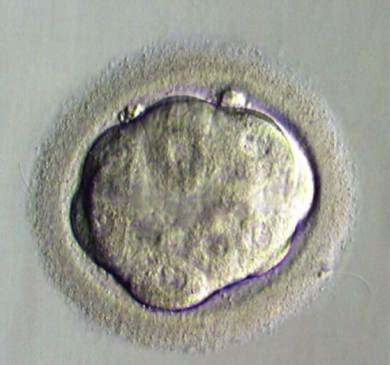
\includegraphics[width=3.6cm]{Figuras/seg4.jpg} & \pause 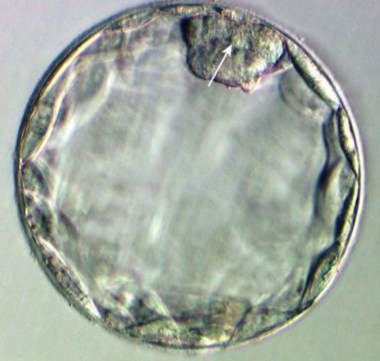
\includegraphics[width=3.6cm]{Figuras/seg5.jpg} & \pause 
		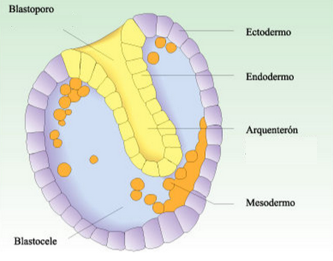
\includegraphics[width=3.6cm,height=3.4cm]{Figuras/blastoporo2.jpg}
	\end{tabular}
\end{frame}

%----------Diapositiva 3 Gastrulacion
\begin{frame}
	\frametitle{Gastrulaci\'on}
	\centering
	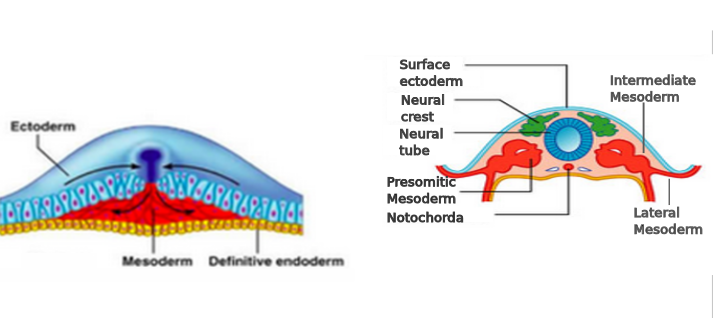
\includegraphics[width=11cm]{Figuras/gastrulacion.png}
\end{frame}

\begin{frame}
	\frametitle{Somitog\'enesis}
	\centering
	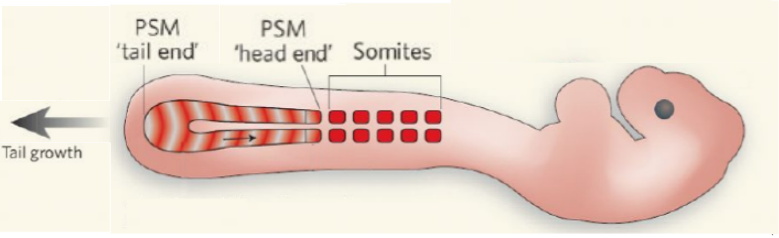
\includegraphics[width=10cm]{Figuras/somitogenesis2inv.png} \pause \\[.1cm]
	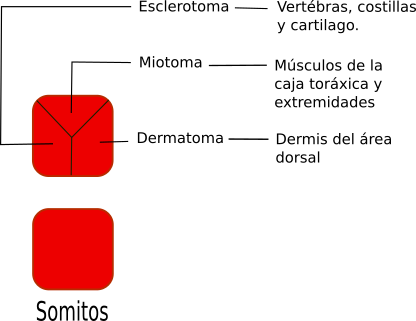
\includegraphics[width=6cm]{Figuras/somito.png}
	
\end{frame}
\begin{frame}{somitog\'enesis}
	\centering
	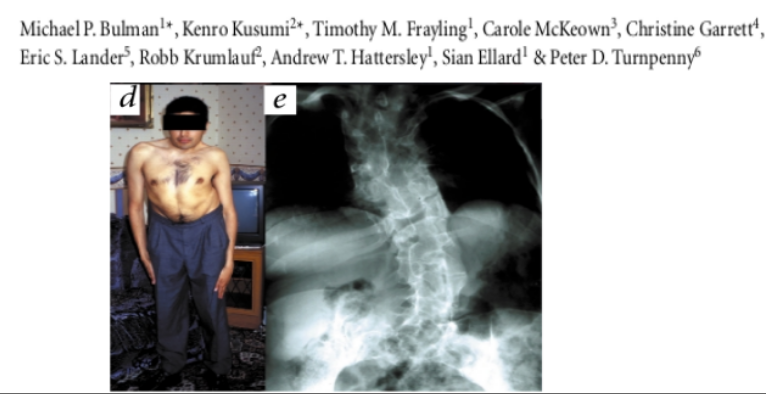
\includegraphics[width=8cm]{Figuras/somitogenesis3.png} \\[.2cm]
	\pause
	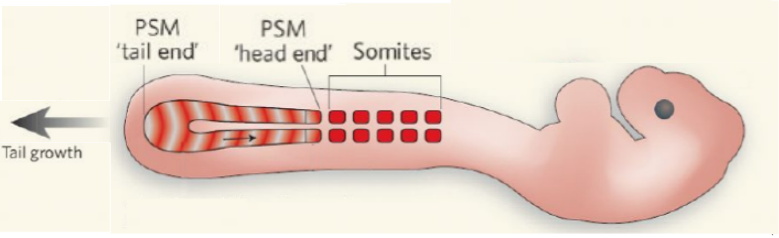
\includegraphics[width=9cm]{Figuras/somitogenesis2inv.png}
\end{frame}	


\begin{frame}{Antecedentes}
	\centering
	\includegraphics[width=8cm, height=3.5cm]{Figuras/escalas2.pdf}
	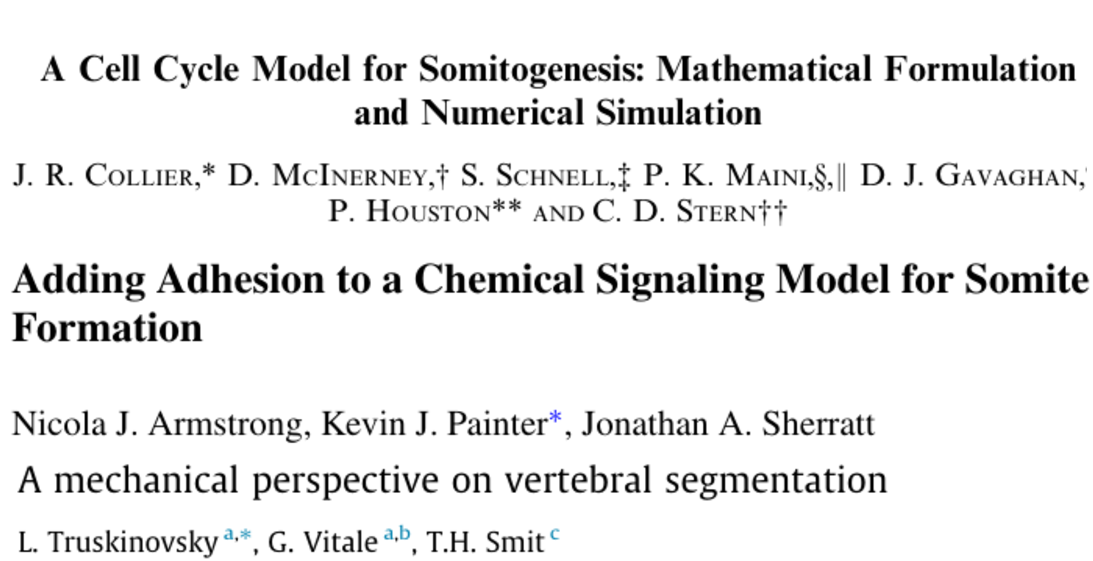
\includegraphics[width=8cm]{Figuras/SomitogenesisModels.pdf}
\end{frame}

\begin{frame}
	\frametitle{Modelo de reloj y frente de onda}
	\centering
	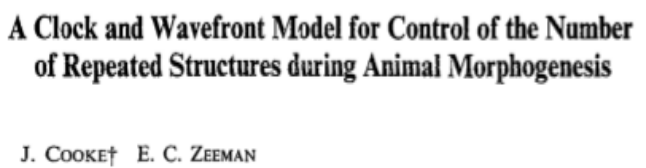
\includegraphics[width=10cm]{Figuras/FO.png} \\[.5cm]
	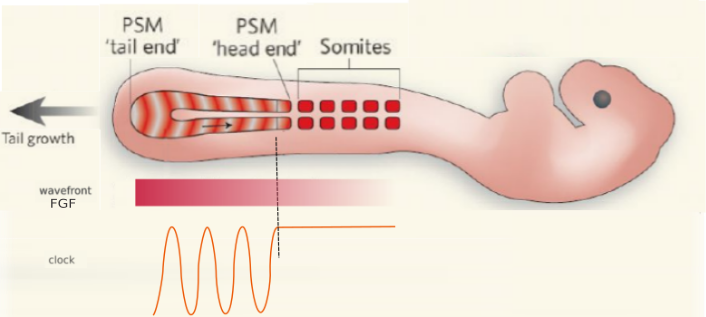
\includegraphics[width=10cm]{Figuras/FOinv.png}
\end{frame}


\begin{frame}
	\frametitle{Antecedentes modelo de reloj y frente de onda}% Genes con expresi\'on c\'iclica
	\centering
	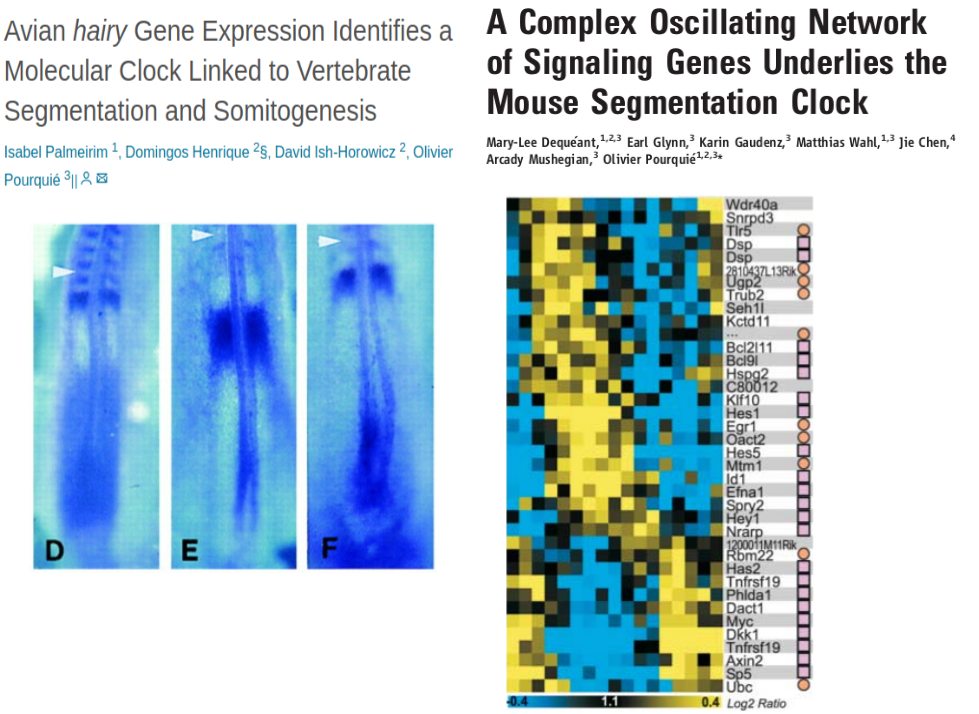
\includegraphics[width=10cm]{Figuras/antecedentesFO3.png}
\end{frame}


%------------Diapositiva 7
\begin{frame}
	\frametitle{Gradientes de concentraciones candidatos a ser el FO}
	\centering
	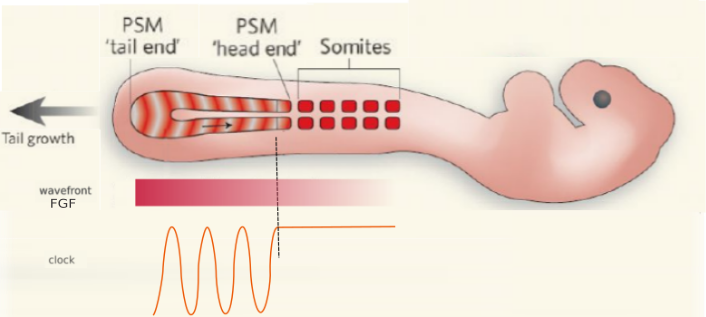
\includegraphics[width=7cm]{Figuras/FOinv.png} \\
	\vspace{.3cm}
	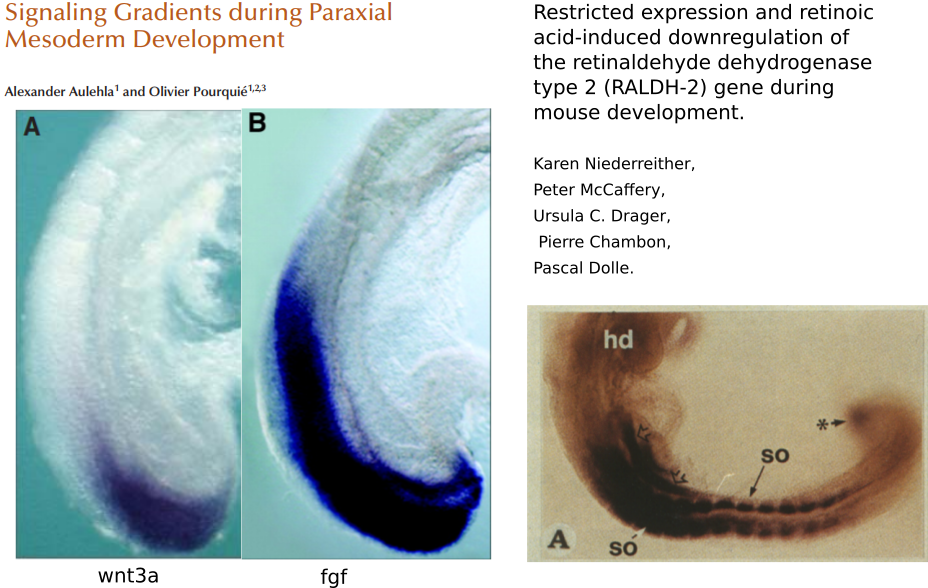
\includegraphics[width=8cm,height=4cm]{Figuras/antecedentesFO4.png} \\[.cm]
	%\pause

\end{frame}

\begin{frame}
	\frametitle{Antecedentes modelo de reloj y frente de onda}
	\centering
	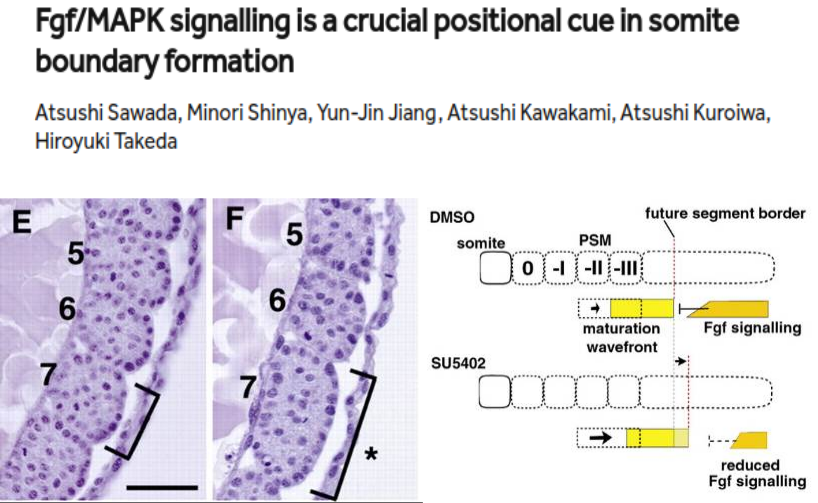
\includegraphics[width=10cm]{Figuras/antecedentesFO5.png}
	
\end{frame}

\begin{frame}
	\frametitle{Antecedentes modelo de reloj y frente de onda}
	\centering %\pause
	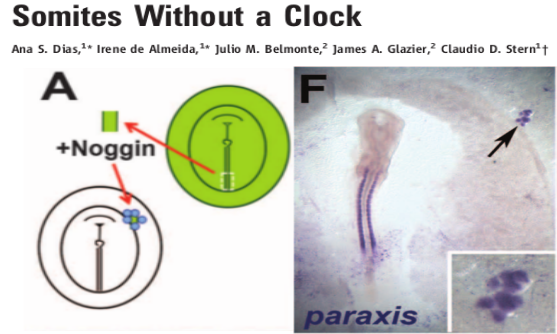
\includegraphics[width=7cm]{Figuras/antecedentesFO2.png} \\
	\pause
	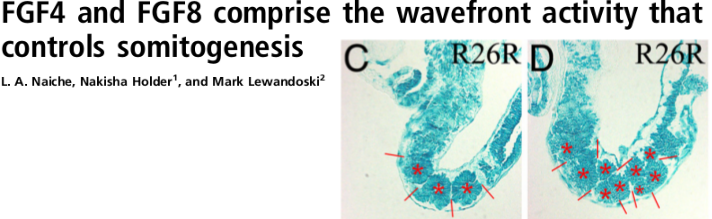
\includegraphics[width=10cm]{Figuras/antecedentesFO1.png}
	
\end{frame}
\begin{frame}{Modelos de reacción-difusión}
	\centering
	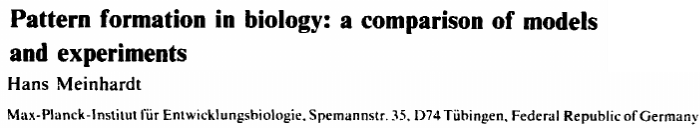
\includegraphics[width=10cm]{Figuras/Meinhardt.png}
	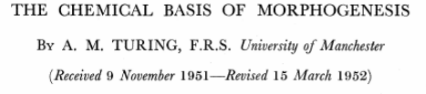
\includegraphics[width=10cm]{Figuras/turing.png} \\[.3cm]

	\pause
	
	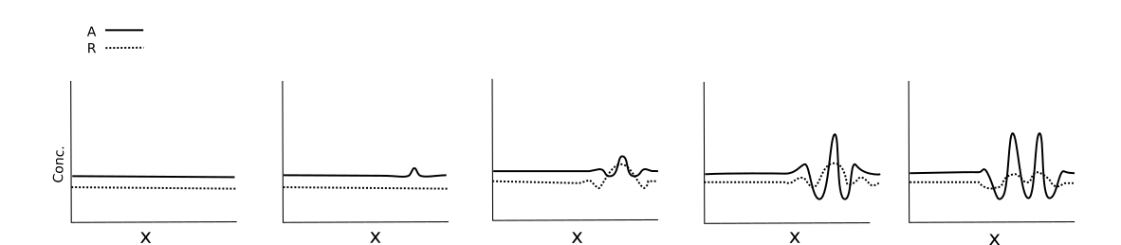
\includegraphics[width=10cm]{Figuras/explicacionRD}
\end{frame}



%------------Diapositiva 19
\begin{frame}
	\frametitle{Modelo PORD}
	\centering
	%\pause
	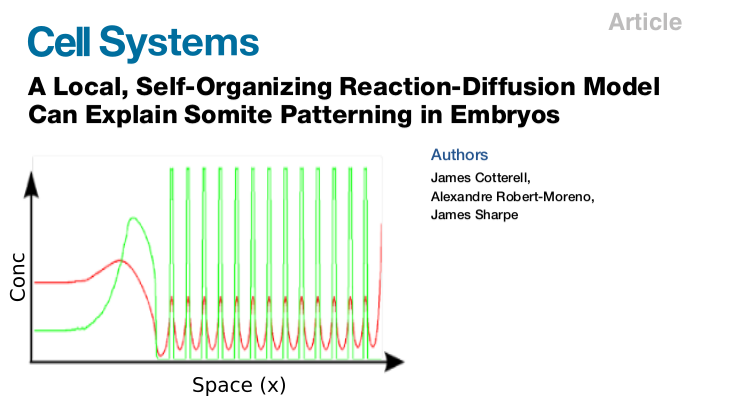
\includegraphics[width=9cm]{Figuras/reaction-difusion.png} \\ 
	\pause
	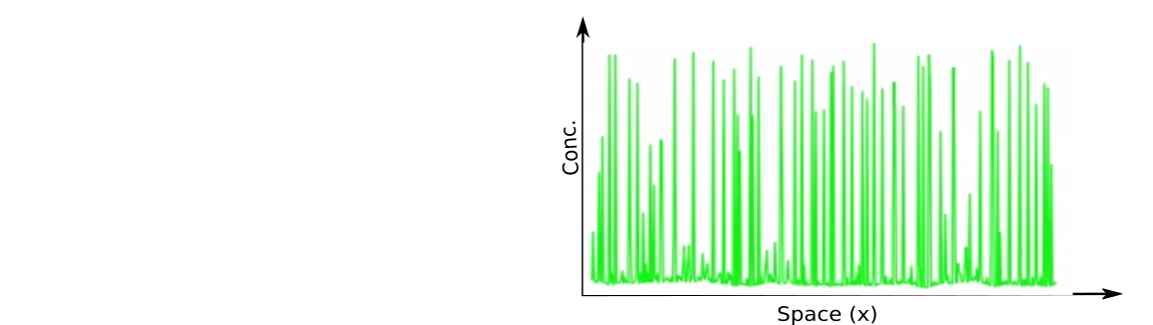
\includegraphics[width=9cm]{Figuras/reaction-difusion3.png}
\end{frame}


\begin{frame}
	\frametitle{Planteamiento del problema}
	\begin{table}
		
	\begin{tabular}{c c}
	\centering
	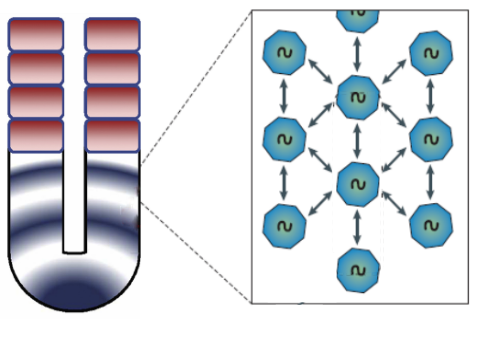
\includegraphics[width=5cm]{Figuras/Diapo14d} & 	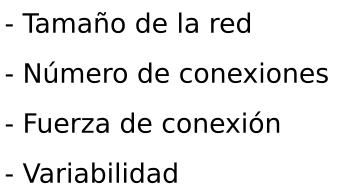
\includegraphics[width=4cm]{Figuras/Diapo14e} \\ %\vspace{.5cm}
	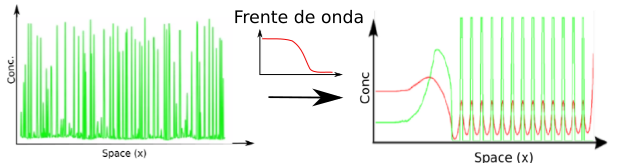
\includegraphics[width=6cm]{Figuras/Diapo14b}  
	
	
\end{tabular}
\end{table}
\end{frame}

%------------Diapositiva 20
\begin{frame}
	\frametitle{Hip\'otesis} 
	\begin{block}{Hip\'otesis}
	La robustez espacio-temporal de la somitogénesis es afectada por interacciones a escala del tejido e interacciones a escala celular.
	
	\end{block}
\end{frame}

\begin{frame}
	\frametitle{Objetivos}
	\begin{block}{Objetivo General}
	Estudiar la dinámica espacio-temporal de la somitogénesis mediante dos modelos a diferente escala, uno a escala del tejido y otro a escala celular.
	
	\end{block}
	\pause
	\begin{block}{Objetivos Particulares}
		\begin{itemize}
		
			\item Estudiar la somitogénesis con un modelo a escala del tejido y analizar su estabilidad para caracterizar su robustez ante diferentes variaciones.
			\item Estudiar con un modelo a escala celular como el número de células, el nivel de conectividad, la fuerza de conexión y la variabilidad celular afectan la sincronización de las células del MPS.	
		
		\end{itemize}
	\end{block}
\end{frame}

%------------Diapositiva 21

\begin{frame}{Metodología}
	\centering
	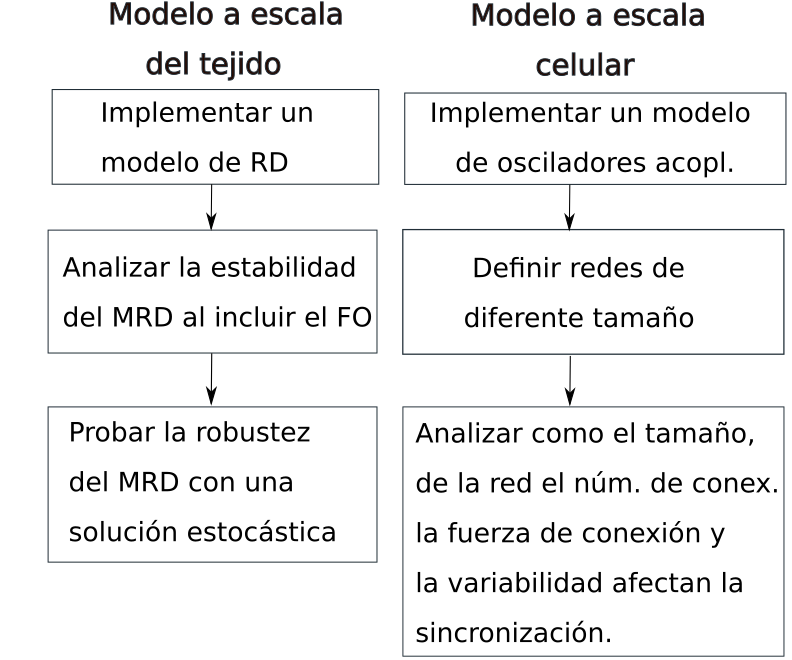
\includegraphics[width=3.5in]{Figuras/metodologia.png}
	
\end{frame}

\begin{frame}{Desarrollo del modelo}
	\centering
	
	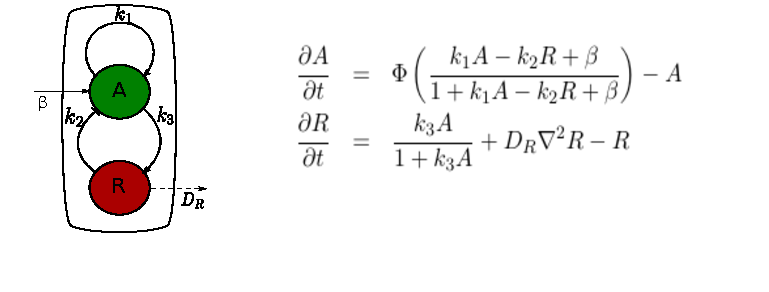
\includegraphics[width=9.5cm]{Figuras/RDT5_1.pdf}
	%\pause
	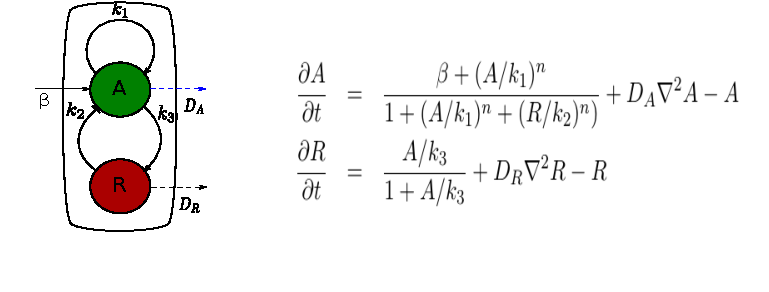
\includegraphics[width=9.5cm]{Figuras/RDT5_2.pdf}
	%\pause
	
\end{frame}

%------------Diapositiva 22

\begin{frame}
	\frametitle{Estimación de los parámetros}
	\centering
	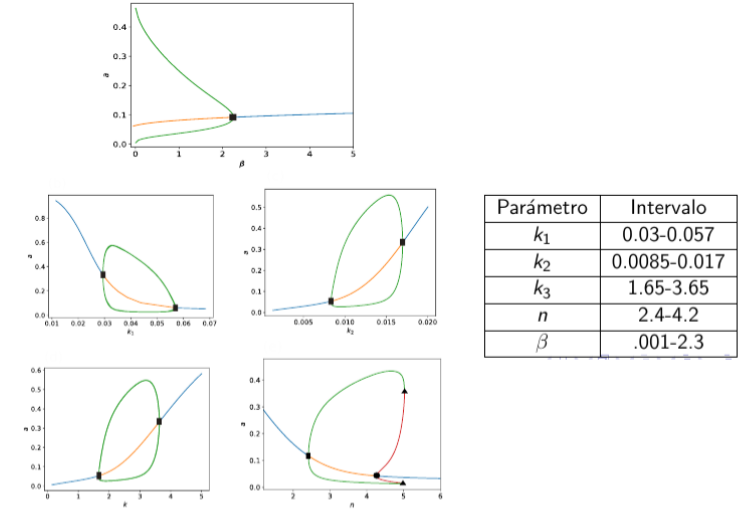
\includegraphics[width=11cm]{Figuras/hopf.png}
	
\end{frame}


\begin{frame}{Resultados. Validación del modelo.}
	\begin{center}
		$k_1=0.05, k_2=0.01, k_3=2.0, \beta=0.5, n=3.0, D_R=0.0025$
		\begin{tikzpicture}[scale = 5] %[remember picture,overlay] 
		\node[anchor=south west, inner sep=0pt] at (current page.south west) {%
			
			\movie[%
			height = .5\paperheight,%
			width = .5\paperwidth,%
			poster,%
			showcontrols]{}{Figuras/movie.mp4}%
		}; 
		\end{tikzpicture}
	\end{center}
\end{frame}

\begin{frame}{Resultados. Validación del modelo.}
	\centering
	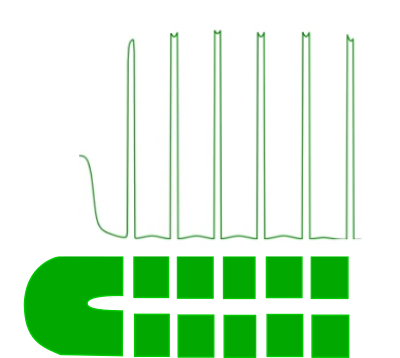
\includegraphics[width=7cm]{Figuras/res1.png}
\end{frame}

%------------Diapositiva 25


\begin{frame}
	\frametitle{An\'alisis de estabilidad espacio-temporal}
	\centering
	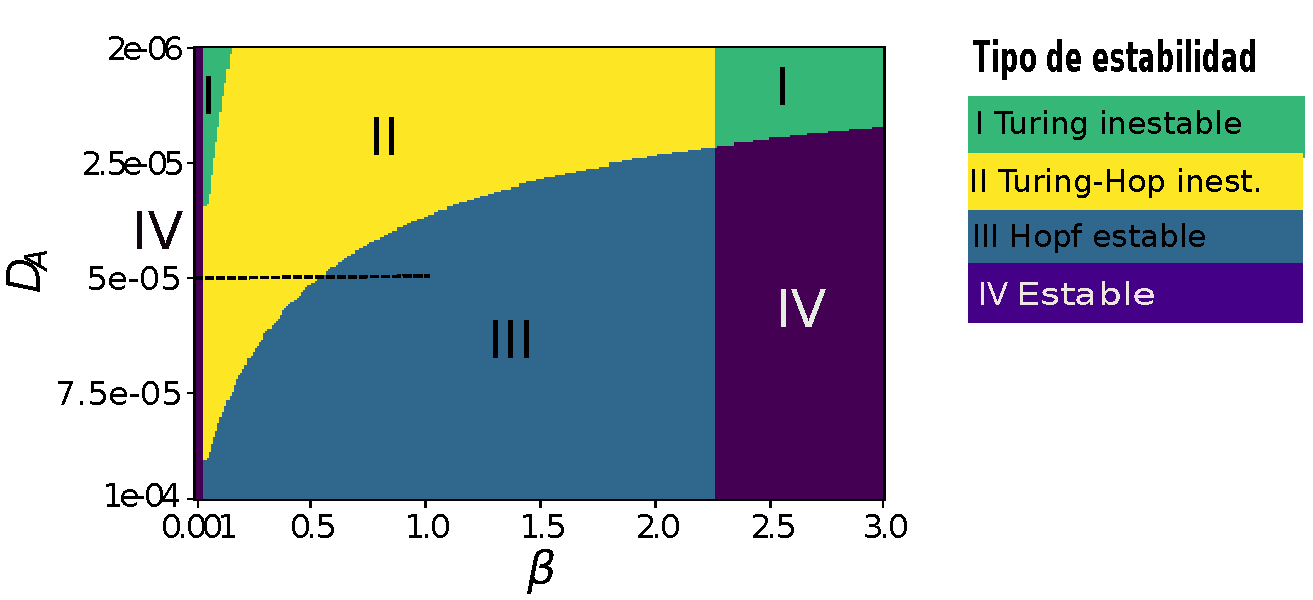
\includegraphics[width=9.5cm]{Figuras/EspParametros.pdf}
\end{frame}
%------------Diapositiva 17
\begin{frame}{Resultados con $\beta$ = 0.1}
	\centering
	\begin{tikzpicture}[scale = 5] %[remember picture,overlay] 
	\node[anchor=south west, inner sep=0pt] at (current page.south west) {%
		
		\movie[%
		height = .5\paperheight,%
		width = .5\paperwidth,%
		poster,%
		showcontrols]{}{Figuras/MovieFigure3A.mp4}
	}; 
	\end{tikzpicture}
	
\end{frame}

\begin{frame}{Resultados $\beta$ = 0.1}
	\centering
	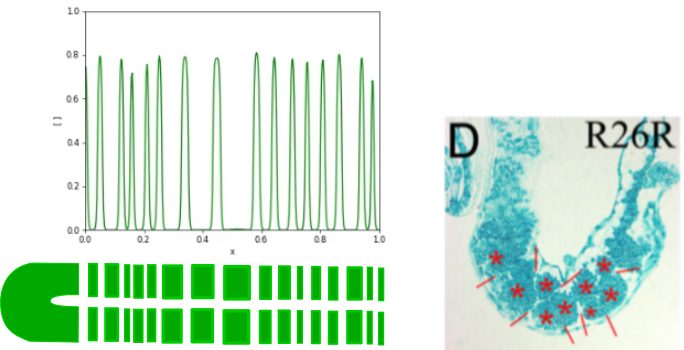
\includegraphics[width=10cm]{Figuras/resbeta_01.png}
	
\end{frame}

%------------Diapositiva 18
\begin{frame}{Resultados con $\beta$ = 0.7}
	\centering
	\begin{tikzpicture}[scale = 5] %[remember picture,overlay] 
	\node[anchor=south west, inner sep=0pt] at (current page.south west) {%
		
		\movie[%
		height = .5\paperheight,%
		width = .5\paperwidth,%
		poster,%
		showcontrols]{}{Figuras/MovieFigure3B.mp4}
	}; 
	\end{tikzpicture}
	
\end{frame}


\begin{frame}{Efecto del FO v= 0.02}
	\centering
	$\beta = f(x,vt) = \frac{k^n}{k^n+(x-vt)^n}$ \\
	\begin{tikzpicture}[scale = 5] %[remember picture,overlay] 
	\node[anchor=south west, inner sep=0pt] at (current page.south west) {%
		
		\movie[%
		height = .5\paperheight,%
		width = .5\paperwidth,%
		poster,%
		showcontrols]{}{Figuras/MovieFigure4A_4B.mp4}
	}; 
	\end{tikzpicture}
\end{frame}


\begin{frame}
	\frametitle{Efecto del FO con v=0.04}
	\centering
	\begin{tikzpicture}[scale = 5] %[remember picture,overlay] 
	\node[anchor=south west, inner sep=0pt] at (current page.south west) {%
		
		\movie[%
		height = .5\paperheight,%
		width = .5\paperwidth,%
		poster,%
		showcontrols]{}{Figuras/MovieFigure4C_4D.mp4}
	}; 
	\end{tikzpicture}
	
	
\end{frame}

\begin{frame}{Tamaño de los somitas en función de la velocidad del FO}
	
	\centering
	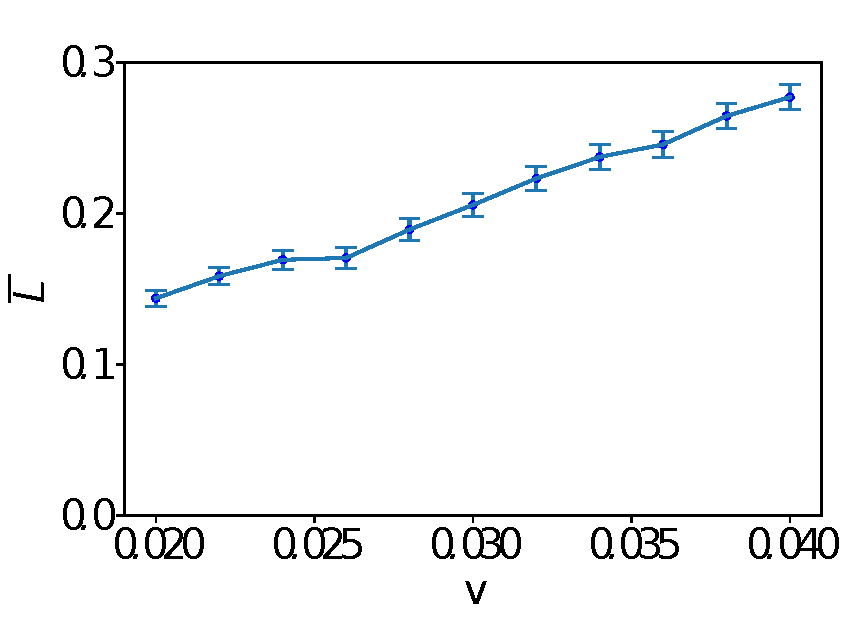
\includegraphics[width=3in]{Figuras/Fig04_2a}
\end{frame}

\begin{frame}{Robustez del tamaño de los somitas en función de la variabilidad en las CI}
	\centering
	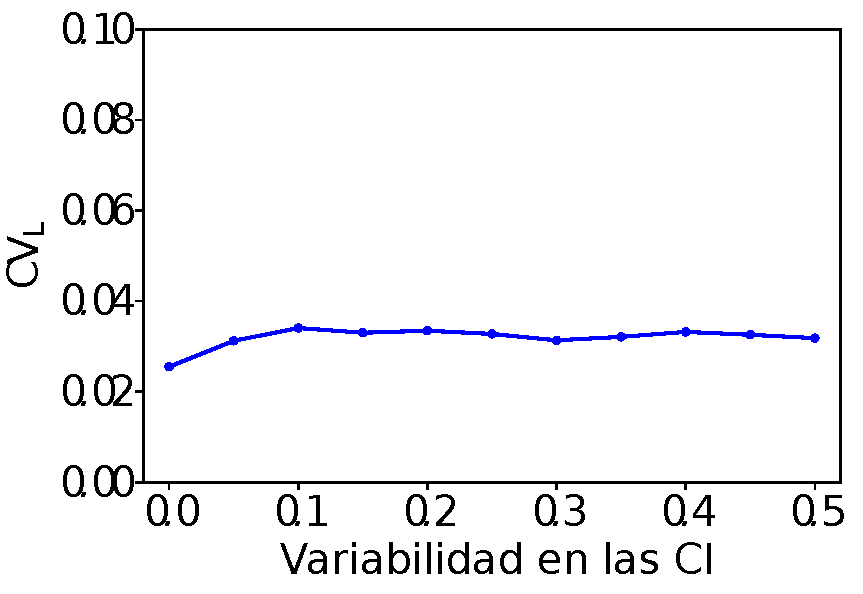
\includegraphics[width=3in]{Figuras/Fig06}
\end{frame}

\begin{frame}
	\frametitle{Robustez al ruido con CV=5\%}
	\centering
	\centering
	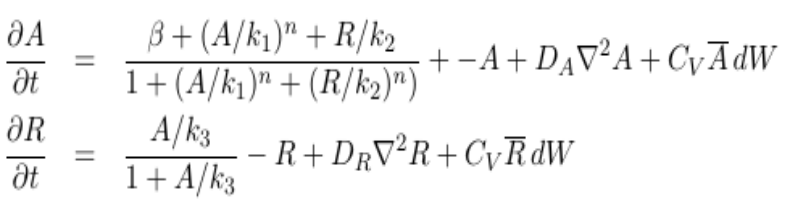
\includegraphics[width=7cm]{Figuras/ecsEstocasticas.png}
	
	\begin{tikzpicture}[scale = 5] %[remember picture,overlay] 
	\node[anchor=south west, inner sep=0pt] at (current page.south west) {%
		
		\movie[%
		height = .5\paperheight,%
		width = .5\paperwidth,%
		poster,%
		showcontrols]{}{Figuras/MovieFigure5A.mp4}
	}; 
	\end{tikzpicture}
\end{frame}

\begin{frame}
	\frametitle{Robustez al ruido con CV=10\%}
	\centering
	\begin{tikzpicture}[scale = 5] %[remember picture,overlay] 
	\node[anchor=south west, inner sep=0pt] at (current page.south west) {%
		
		\movie[%
		height = .5\paperheight,%
		width = .5\paperwidth,%
		poster,%
		showcontrols]{}{Figuras/MovieFigure5B.mp4}
	}; 
	\end{tikzpicture}
\end{frame}

\begin{frame}{Robustez del tamaño de los somitas en función del ruido}
	\centering
	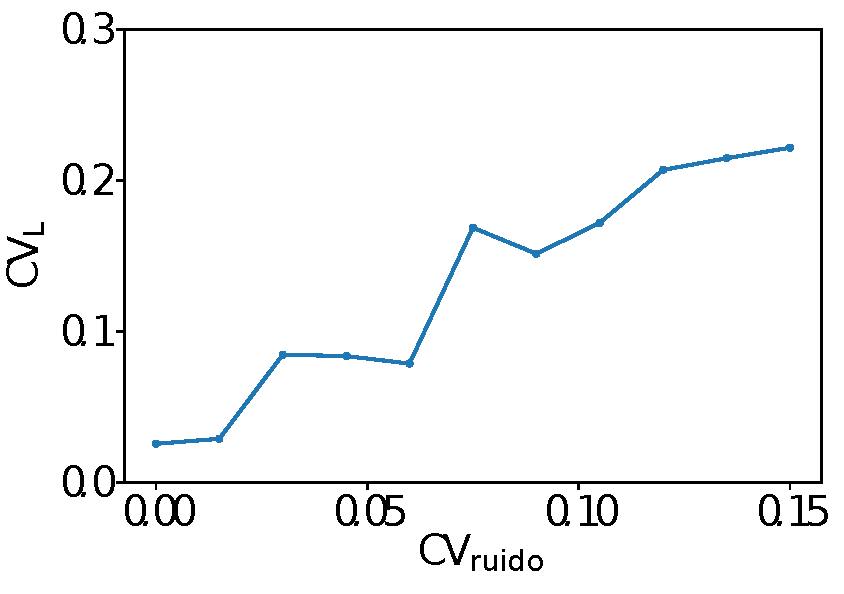
\includegraphics[width=3.0in]{Figuras/Fig06_3}
\end{frame}


\begin{frame}{Discusión MET}
	
	\begin{itemize}
		\item El acoplamiento del frente de onda con el modelo a escala del tejido permiten eliminar la sensibilidad así como la dependencia de las condiciones iniciales, sin embargo, no son suficientes para explicar la robustez que exhibe la somitogénesis.
		\item Es posible que las interacciones a corto alcance involucradas en al sincronización de las células del MPS contribuyan en la robustez.
		
	\end{itemize}
\end{frame}


%------------Diapositiva 5
\begin{frame}
	\frametitle{Estudio a Escala celular, reloj de segmentaci\'on}
	\centering 
	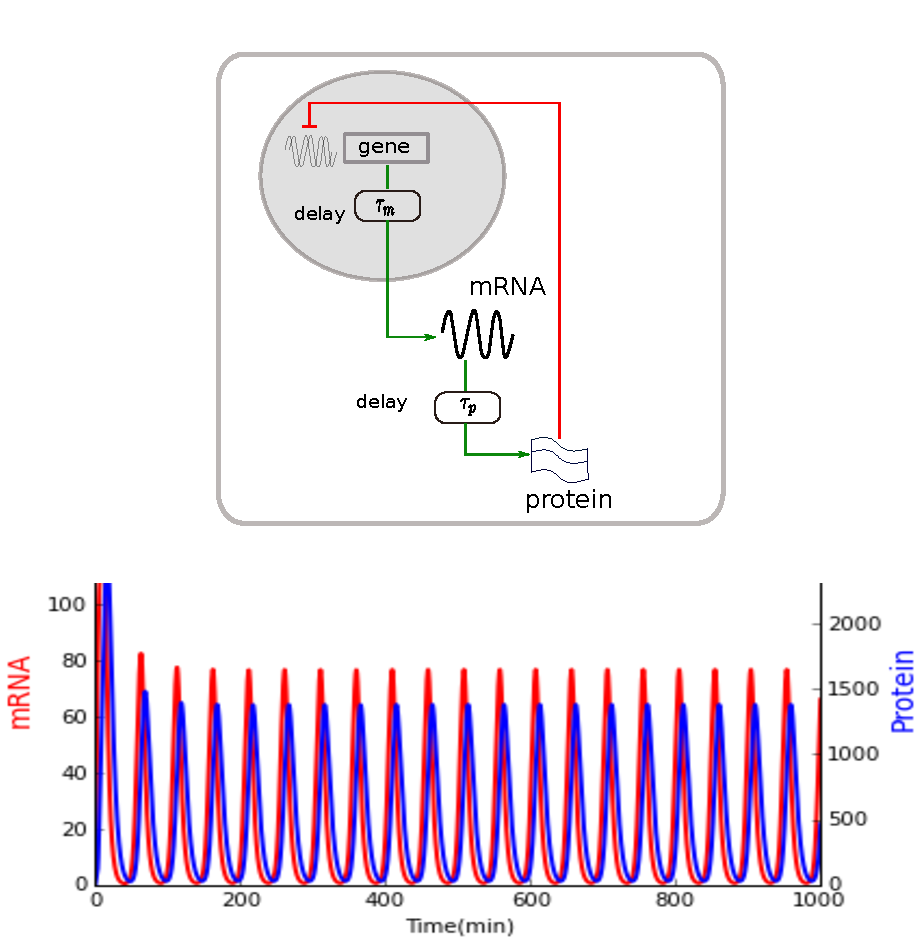
\includegraphics[width=6cm]{Figuras/reloj.pdf} %{reloj.eps}
	\pause
	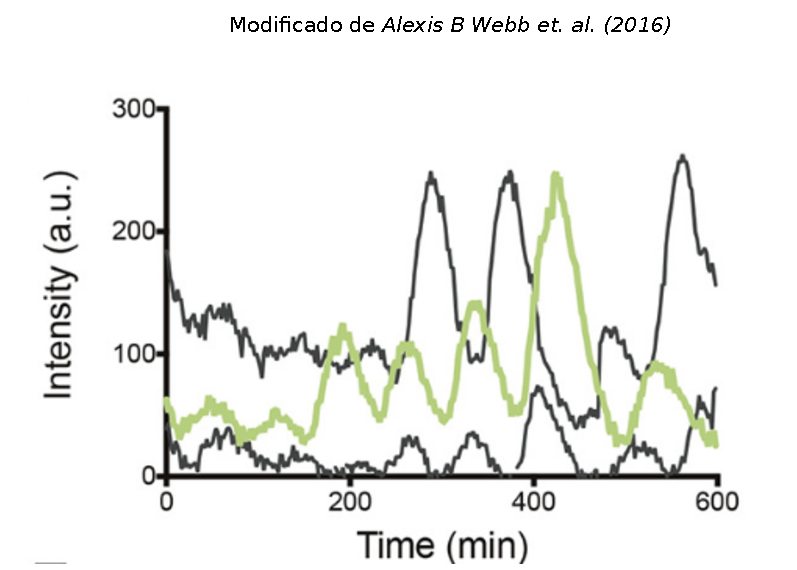
\includegraphics[width=5.5cm]{Figuras/oscilacionEsto.pdf}
\end{frame}

%------------Diapositiva 6
\begin{frame}
	\frametitle{Vía Delta-Notch y sincronizaci\'on}
	\centering
	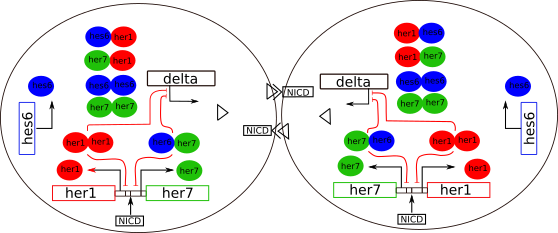
\includegraphics[width=10cm]{Figuras/interactions3.png}
\end{frame}


%------------Diapositiva 9
\begin{frame}
	\frametitle{Desarrollo del modelo a escala celular}
	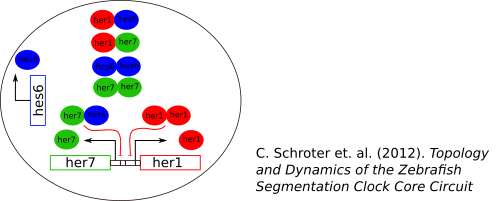
\includegraphics[width=7cm]{Figuras/oscilationsref.png}
	\begin{scriptsize}
		\centering
		\begin{align*}
		\frac{dH_1(t)}{dt} &= \rho_1 \frac{1}{1+(\frac{H_{11}(t-\tau_1)}{k_{11}} + \frac{H_{76}(t-\tau_1)}{k_{76}})^2}-c_1H_1(t) \\ & \hspace{.25cm}-2a_{11}H_1(t)^2 + 2b_{11}H_{11}(t)-a_{16}H_1(t)H_6(t)+b_{16}H_{16}(t)-a_{17}H_1(t)H_7(t)+b_{17}H_{17}(t) \\ %-------
		\frac{dH_6(t)}{dt} &= \rho_6 -c_6H_6(t) \\ & \hspace{.25cm} -2a_{66}H_6(t)^2 + 2b_{66}H_{66}(t)-a_{16}H_1(t)H_6(t)+b_{16}H_{16}(t)-a_{67}H_6(t)H_7(t)+b_{67}H_{67}(t) \\ %-----
		\frac{dH_7(t)}{dt} &= \rho_7 \frac{1}{1+(\frac{H_{11}(t-\tau_7)}{k_{11}} + \frac{H_{76}(t-\tau_7)}{k_{76}})^2}-c_7H_7(t) \\ & \hspace{.25cm}-2a_{77}H_7(t)^2 + 2b_{77}H_{77}(t)-a_{76}H_7(t)H_6(t)+b_{76}H_{76}(t)-a_{17}H_1(t)H_7(t)+b_{17}H_{17}(t)  
		\end{align*}
	\end{scriptsize}
\end{frame}


%------------Diapositiva 10
\begin{frame}
	\frametitle{Modelo base con prote\'ina Delta}
	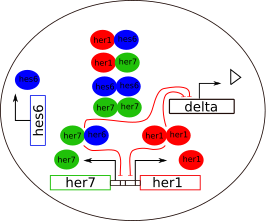
\includegraphics[width=3cm]{Figuras/oscilationsDelta.png}
	\begin{scriptsize}
		\centering
		\begin{align*}
		\frac{dH_1(t)}{dt} &= \rho_1 \frac{1}{1+(\frac{H_{11}(t-\tau_1)}{k_{11}} + \frac{H_{76}(t-\tau_1)}{k_{76}})^2}-c_1H_1(t) \\ & \hspace{.25cm}-2a_{11}H_1(t)^2 + 2b_{11}H_{11}(t)-a_{16}H_1(t)H_6(t)+b_{16}H_{16}(t)-a_{17}H_1(t)H_7(t)+b_{17}H_{17}(t) \\ %-------
		\frac{dH_6(t)}{dt} &= \rho_6 -c_6H_6(t) \\ & \hspace{.25cm} -2a_{66}H_6(t)^2 + 2b_{66}H_{66}(t)-a_{16}H_1(t)H_6(t)+b_{16}H_{16}(t)-a_{67}H_6(t)H_7(t)+b_{67}H_{67}(t) \\ %-----
		\frac{dH_7(t)}{dt} &= \rho_7 \frac{1}{1+(\frac{H_{11}(t-\tau_7)}{k_{11}} + \frac{H_{76}(t-\tau_7)}{k_{76}})^2}-c_7H_7(t) \\ & \hspace{.25cm}-2a_{77}H_7(t)^2 + 2b_{77}H_{77}(t)-a_{76}H_7(t)H_6(t)+b_{76}H_{76}(t)-a_{17}H_1(t)H_7(t)+b_{17}H_{17}(t) \\
		\frac{dD(t)}{dt} &= \rho_D \frac{1}{1+(\frac{H_{11}(t-\tau_D)}{k_{11}} + \frac{H_{76}(t-\tau_D)}{k_{76}})^2}-c_DD(t) \end{align*}
	\end{scriptsize}
\end{frame}

%------------Diapositiva 11
\begin{frame}
	\frametitle{Normalizaci\'on del modelo}
	
	\begin{align*}
	a_{\mu\nu} &=a, b_{\mu\nu}=b, c_{\mu\nu}=c,k_{\mu\nu} = k \\
	\alpha &= ak/c, \beta=b/c, \gamma_i =\rho_i \delta /ck,  s=ct \\
	H_{\mu\nu}(t) &=\delta H_{\mu}(t)H_{\nu}(t) , \delta = (\alpha/(1+\beta))^{1/2} \\
	\end{align*}
	\begin{tiny}
	\begin{align*}
	\frac{dh_1(s)}{ds} &= \gamma_1\frac{1}{1 + (h_1(s-\tau_1))^2+h_7(s-\tau_1)h_6(s-\tau_1))^2} - h_1(s)-\delta(h_1(s)(2h_1(s)+h_6(s)+h_7(s)) \\
	\frac{dh_6(s)}{ds} &= \gamma_6-h_6(s) - \delta h_6(s)(h_1(s)+2h_6(s)+h_7(s)) \\
	\frac{dh_7(s)}{ds} &= \gamma_7\frac{1}{1 + (h_1(s-\tau_7))^2+h_7(s-\tau_7)h_6(s-\tau_7))^2} - h_7(s)-\delta(h_7(s)(h_1(s)+h_6(s)+2h_7(s)) \\
	\frac{dD(s)}{ds} &= \gamma_D\frac{1}{1 + (h_1(s-\tau_D))^2+h_7(s-\tau_D)h_6(s-\tau_D))^2} - D(s)
	\end{align*}
\end{tiny}
\end{frame}

%------------Diapositiva 12
\begin{frame}
	\frametitle{Ecuaciones para la interacci\'on entre varias células}
	\centering
	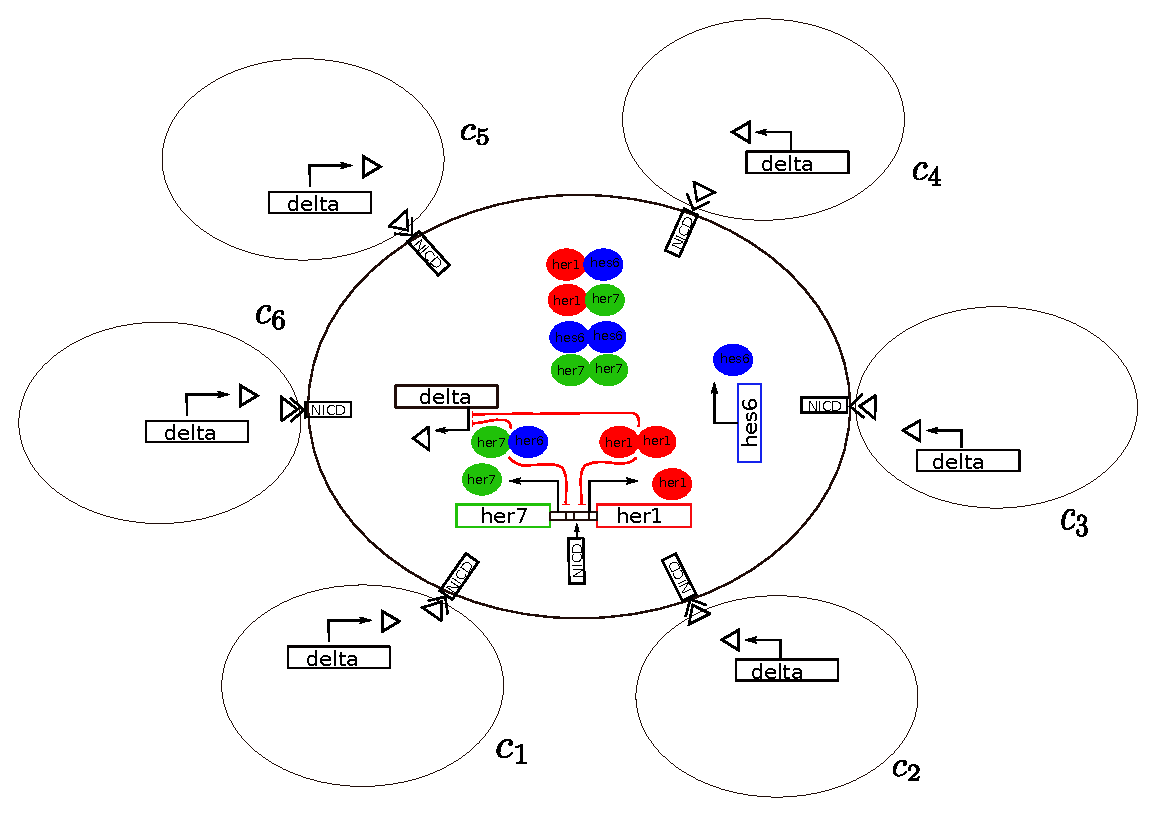
\includegraphics[width=6cm]{Figuras/interactionsMultipleSimple.eps} 
	\begin{tiny}
	\begin{align*}
	\frac{dh_1(s)}{ds} &= \gamma_1\frac{1}{1 + (h_1(s-\tau_1))^2+h_7(s-\tau_1)h_6(s-\tau_1))^2}(g(\sum_{j}D_j)) - h_1(s)-\delta(h_1(s)(2h_1(s)+h_6(s)+h_7(s)) \\
	\frac{dh_6(s)}{ds} &= \gamma_6-h_6(s) - \delta h_6(s)(h_1(s)+2h_6(s)+h_7(s)) \\
	\frac{dh_7(s)}{ds} &= \gamma_7\frac{1}{1 + (h_1(s-\tau_7))^2+h_7(s-\tau_7)h_6(s-\tau_7))^2}(g(\sum_{j}D_j)) - h_7(s)-\delta(h_7(s)(h_1(s)+h_6(s)+2h_7(s)) \\
	\frac{dD(s)}{ds} &= \gamma_D\frac{1}{1 + (h_1(s-\tau_D))^2+h_7(s-\tau_D)h_6(s-\tau_D))^2} - D(s) 
	\end{align*}
	$g(D) = \frac{D^2}{k_D^2+D^2}$
	\end{tiny}
\end{frame}


\begin{frame}
	\frametitle{Niveles de conexi\'on}
	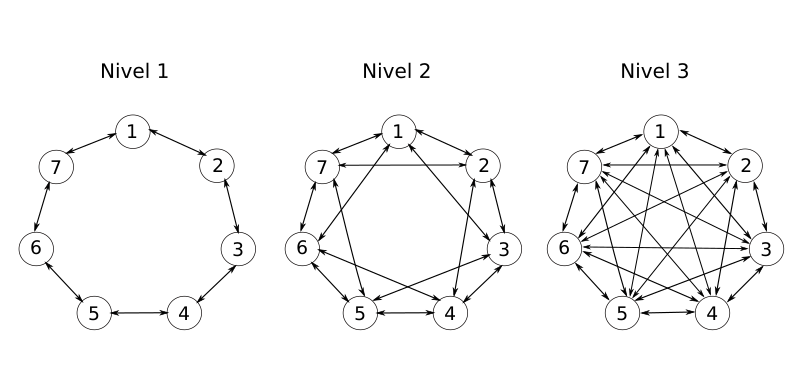
\includegraphics[width = 12cm]{Figuras/niveles.png}
\end{frame}
%------------Diapositiva 13


%------------Diapositiva 14
\begin{frame}
	\frametitle{Parámetro de Orden y par\'ametros del modelo.}
	\centering $R=\frac{Var(M)}{\overline{Var(b_i)}}$
	\pause
	\begin{table}
		\begin{tabular}{|c | c| c|}
			\hline Par\'ametro &Valor & Ref. \\ \hline
			$\gamma_1$ & 10.0 & Scrotter et al. \\ \hline 
			$\gamma_6$ & 25.0 & Scrotter et. al.\\ \hline
			$\gamma_7$ & 10.0 & Scrotter et. al\\ \hline
			$\gamma_D$ & 2.0 & Ahmet et. al. \\ \hline
			$\delta$   & 1.0 & Scrotter et. al. \\ \hline
			$\tau_1 $ & 1.02 & Scrotter et. al.\\ \hline
			$\tau_7 $ & 1.00 & Scrotter et. al.\\ \hline
			$\tau_D $ & 0.85 &Scrotter et. al. \\ \hline
			$k_D $ & 1.0 & Ahmet et. al.\\ \hline
		\end{tabular}
	\end{table}
\end{frame}

%------------Diapositiva 15

\begin{frame}
	\frametitle{Efecto del tamaño de la red y el número de conexiones en la sincronización}
		\centering
		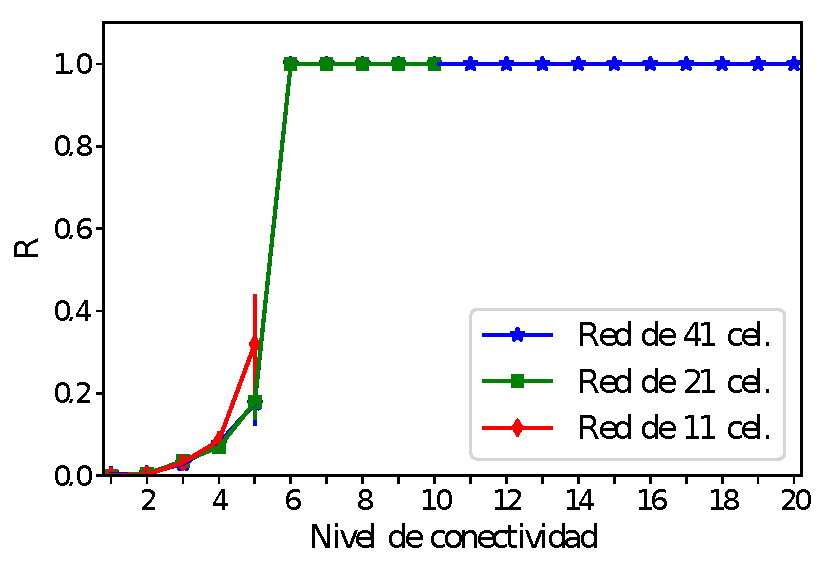
\includegraphics[width=5.0cm]{Figuras/figuraVCIVer533graf.pdf}
		\pause
		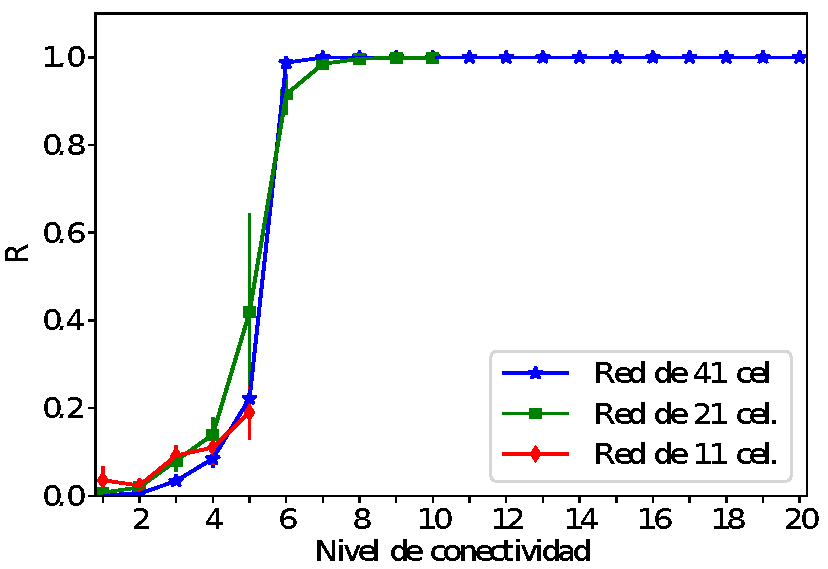
\includegraphics[width=5.0cm]{Figuras/figuraVCIVer1301281273graf.pdf}
\end{frame}

\begin{frame}
	\begin{center}
		\frametitle{Progresi\'on de la sincronizaci\'on}
		
		\begin{tabular}{c c}
			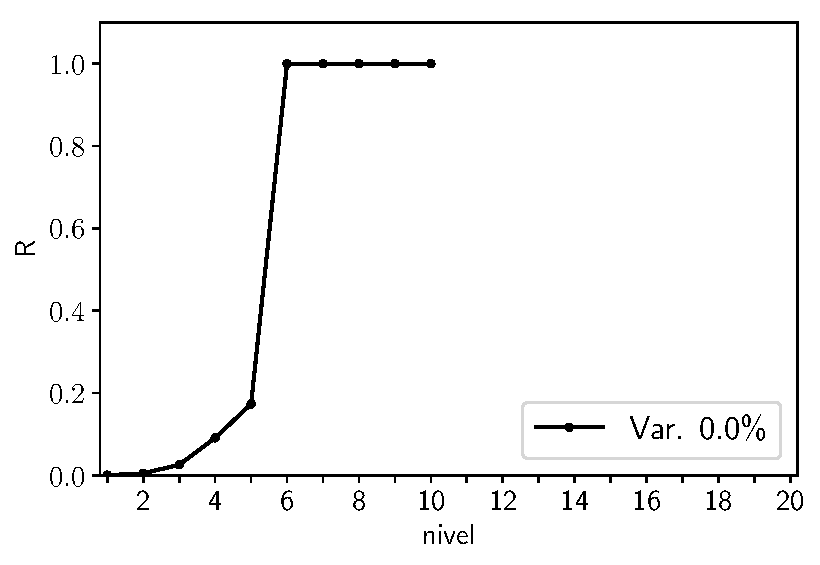
\includegraphics[width = 4.5cm]{Figuras/figuraVCIVer71Unico_.pdf} & 
			\begin{tikzpicture}[scale = 3.0] %[remember picture,overlay] 
			\node[anchor=south west, inner sep=0pt] at (current page.south west) {%
				
				\movie[%
				height = .3\paperheight,%
				width = .3\paperwidth,%
				poster,%
				showcontrols]{}{Figuras/presentacion_v53.avi}%
			}; 
			\end{tikzpicture} \\ 
			
		\end{tabular}
	\end{center}\end{frame}


%------------Diapositiva 15
\begin{frame}
\begin{center}
	\frametitle{Efecto de la fuerza de conexión en la sincronización. 11 cel.}
	
	\begin{tabular}{c c}
		\multicolumn{2}{c}{$g(D) = \frac{D^2}{k_D^2+D^2}$; $k_D = \frac{k_{disoc}}{k_{asoc}}$}
		\\
		\begin{tikzpicture}[scale = 2.5] %[remember picture,overlay] 
		\node[anchor=south west, inner sep=0pt] at (current page.south west) {%
			
			\movie[%
			height = .3\paperheight,%
			width = .3\paperwidth,%
			poster,%
			showcontrols]{}{Figuras/movien_3kd_0.32v_49.mp4}%
		}; 
		\end{tikzpicture} & 
		\begin{tikzpicture}[scale = 3.0] %[remember picture,overlay] 
		\node[anchor=south west, inner sep=0pt] at (current page.south west) {%
			
			\movie[%
			height = .3\paperheight,%
			width = .3\paperwidth,%
			poster,%
			showcontrols]{}{Figuras/movien_3kd_1.28v_49.mp4}%
		}; 
		\end{tikzpicture} \\ 
		\begin{tikzpicture}[scale = 3.0] %[remember picture,overlay] 
		\node[anchor=south west, inner sep=0pt] at (current page.south west) {%
			
			\movie[%
			height = .3\paperheight,%
			width = .3\paperwidth,%
			poster,%
			showcontrols]{}{Figuras/movien_3kd_10.24v_49.mp4}%
		}; 
		\end{tikzpicture} &
		
		\includegraphics[width = 4.7cm]{Figuras/figuraVarkdcortadoVer3d_44.pdf} \\ 
	\end{tabular}
\end{center}
\end{frame}

%------------Diapositiva 16
\begin{frame}
\frametitle{Efecto de la fuerza de conexión en la sincronización. 21 y 41 cel.}

\centering
\includegraphics[width=7.5cm]{Figuras/figuraVarkdcortadoVer3d_43.pdf} \\
\includegraphics[width=7.5cm]{Figuras/figuraVarkdcortadoVer3d_42.pdf}

\end{frame}
%\end{comment}

\begin{frame}
	\frametitle{Efecto del parámetro $\gamma_D$ en la sincronización}
	\centering
	\includegraphics[width=4.0cm]{Figuras/figuraVarGdSVer3d_26.pdf} 
	\includegraphics[width=6.0cm]{Figuras/figuraVarGdSVer3d_17.pdf} \\
	\includegraphics[width=8.0cm]{Figuras/figuraVarGdSVer3d_25.pdf}
\end{frame}


\begin{frame}{Robustez de la sincronización ante la variabilidad en las células del MPS.}

\centering
\begin{tabular}{c c}
	\includegraphics[width=5.3cm]{Figuras/figuraVCIVer69_preAv.pdf}&
	\includegraphics[width=5.3cm]{Figuras/figuraVCIVer71_preAv.pdf} 
\end{tabular}
	\includegraphics[width=5.3cm]{Figuras/figuraVCIVer68_preAv.pdf} % cambiar por la corrida para 20 celulas%
\end{frame}

\begin{frame} {Discusión modelo escala celular}
\begin{itemize}
	\item Se requiere de una cantidad mínima de células para que se de la sincronización.
	
	\item La disminución de la fuerza de conexión tiene un efecto negativo en la sincronización, pero este efecto es revertido al aumentar el número de conexiones.
	
	\item {El incremento en el n\'umero de c\'elulas da robustez a la sincronización ante la variabilidad.}
	
	
\end{itemize}
\end{frame}



%------------Diapositiva 18
\begin{frame}{Conclusiones}
	\begin{itemize}
		\item Para explicar la robustez observada en la somitogenesis es necesario considerar las interacciones tanto a escala celular como a escala del tejido.
	\end{itemize}
	
\end{frame}
	


%------------Diapositiva 19
\begin{frame}{Perspectivas}

	\begin{itemize}
		\item Plantear un modelo de reacción-difusión basado en las interacciones de las vías Wnt, FGF y Notch para identificar los posibles componentes que plantea el modelo a escala del tejido.

\end{itemize}
\end{frame}


%------------Diapositiva 32
\begin{frame}
\Huge{\centerline{Gracias.}}
\end{frame}

\end{document}